\documentclass{article}
\usepackage[english]{babel}
\usepackage[utf8x]{inputenc}
\usepackage[fleqn]{amsmath}
\usepackage{amssymb}
\usepackage{graphicx}
\usepackage[colorinlistoftodos]{todonotes}
\usepackage{geometry}
\geometry{hmargin=2.0cm,vmargin=1.5cm}
\usepackage{wrapfig}	% Figures avec du texte autour
\usepackage{lipsum}

\title{Anisotropic equivalent fluid identification}
\author{Arthur TERROIR}
\date{\today}

\begin{document}
\maketitle

%%%%%%%%%%%%%%%%%%%%%%%%%%%%%%%%%%%%%%%%%%%%%%%%%%%%%%%%%%%%%%%%%%%%%%
\section{Introduction}


%%%%%%%%%%%%%%%%%%%%%%%%%%%%%%%%%%%%%%%%%%%%%%%%%%%%%%%%%%%%%%%%%%%%%%
\section{Description of the configuration}
    The material studied is a layer of equivalent fluid, with anisotropic complex density as follow : 
    \begin{align}
        \Bar{\Bar{\rho}}=\begin{pmatrix}
    					\rho_{1} & \rho_{12} & \rho_{13} \\
                        \rho_{12} & \rho_{2} & \rho_{23} \\
                        \rho_{13} & \rho_{23} & \rho_{3}\end{pmatrix}\label{Density_tensor}.
    \end{align}
    The propagation problem is described on the figure (\ref{Schema_PB}), the medium is excited with a acoustic harmonic plane wave on $x_3=L$. The fluid layer is supposed to be infinite along the plan $x_1x_2$ and with a debt L along $x_3$. The incident wave is oriented with two angle , elevation $\theta$ and azimuthal $\phi$, the three projected wave number are :   
   \begin{align}
    &k_1=-k_0 sin(\theta) cos(\phi),\label{k1} \\
    &k_2=-k_0 sin(\theta) sin(\phi),\label{k2} \\
    &k_3= -k_0 cos(\theta),\label{k3}
    \end{align}
    where $k^{(0)}$ is the incident wave number at the radial frequency $\omega$. 
    
    \begin{figure}[ht!]
        \centering
        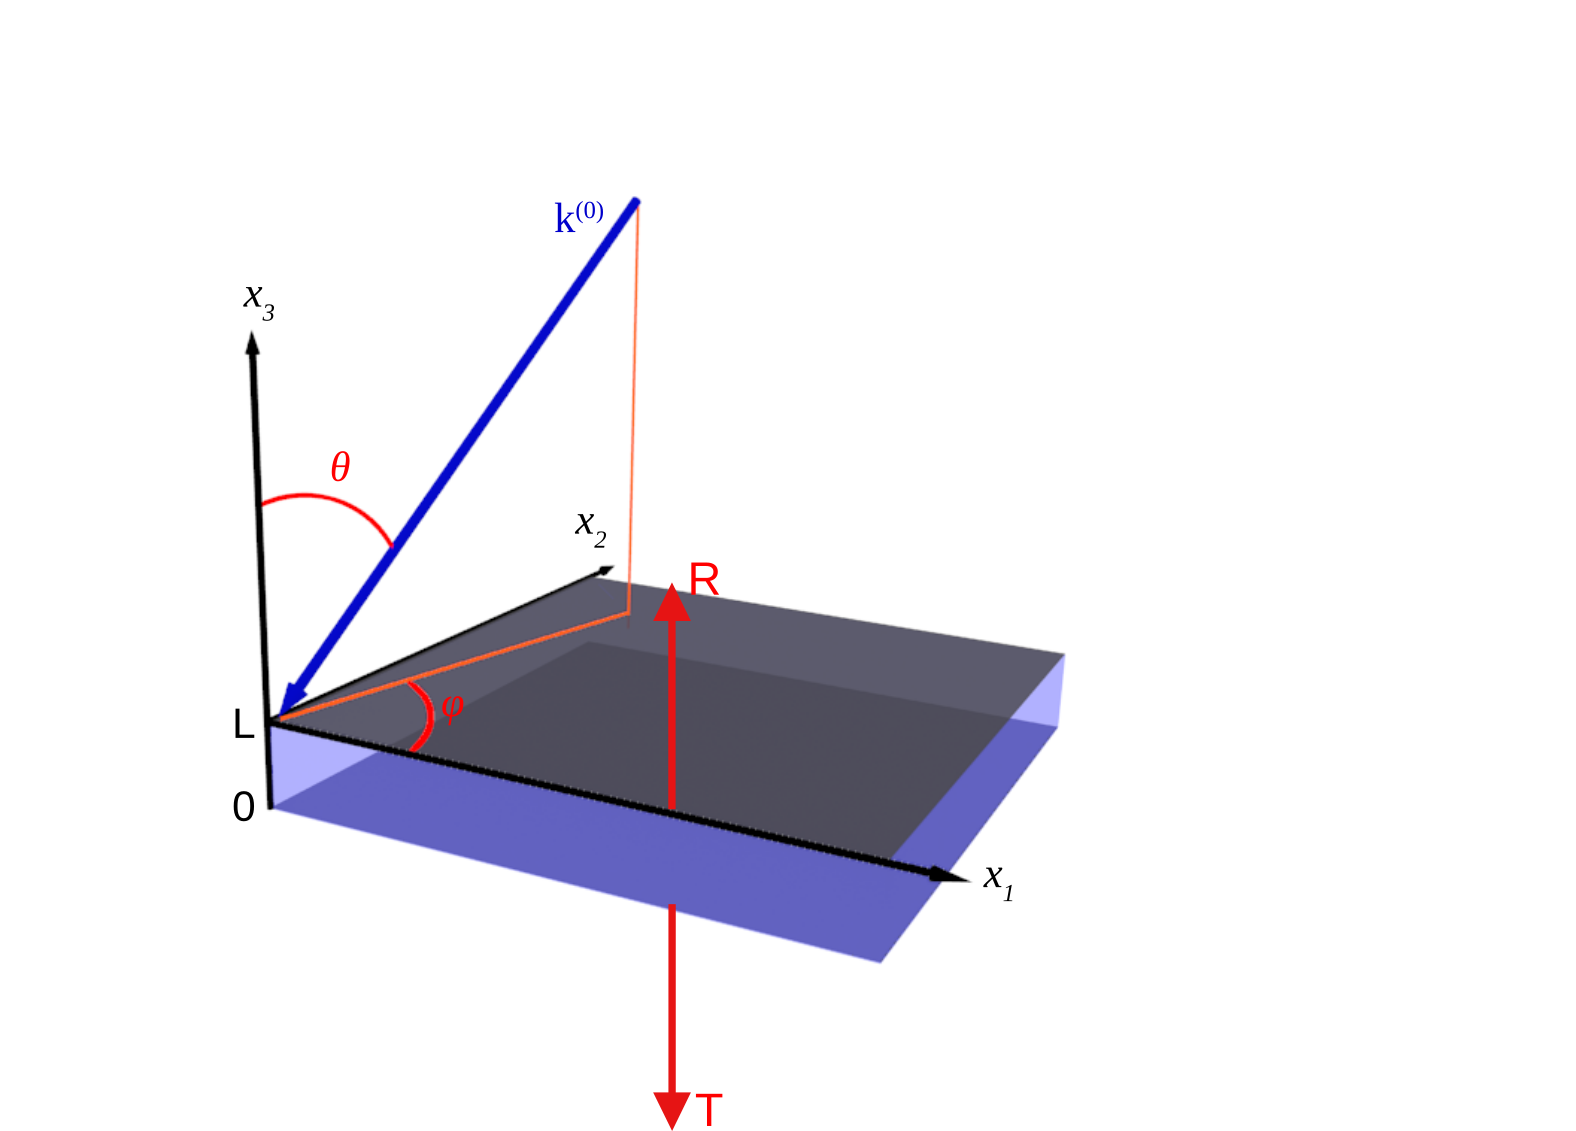
\includegraphics[scale=0.6]{Fig3D.png}
        \caption{azerty}
        \label{Schema_PB}
    \end{figure}
    
    Considering the propagation problem, the boundary condition are defined using the reflection and transmission coefficient, the incident and reflected wave are observed on the interface at $x_3=L$ and the transmitted wave at $x_3=0$, the boundary condition can be write as :
     \begin{align}
    &\bar{S}_{(L)}=\begin{pmatrix}
    	p \\ v_3
    \end{pmatrix}_{(L)}=\begin{pmatrix}
    					    1+R \\ -\frac{k_3}{\rho \omega}(1-R),
    					\end{pmatrix},\label{BC_L} \\
  	&\bar{S}_{(0)}=\begin{pmatrix}
    	p \\ v_3
    \end{pmatrix}_{(0)}=\begin{pmatrix}
    						Te^{ik_3L} \\ -\frac{k_3}{\rho \omega}Te^{ik_3L}
    					\end{pmatrix},\label{BC_0}
    \end{align}                         
    with $\bar{S}$ the state vector (pressure and particle velocity) of the wave propagating, and R and T, the reflection coefficient at $x_3=L$ and the transmission coefficient at $x_3=0$.  
    
%%%%%%%%%%%%%%%%%%%%%%%%%%%%%%%%%%%%%%%%%%%%%%%%%%%%%%%%%%%%%%%%%%%%%%
\section{Parameters identification}
\subsection{Transfer Matrix}
    To achieve the parameters identification, the transfer matrix of the fluid should be known to describe the propagation of the wave between the two interface. It's here proposed to derive the transfer matrix using the following Euler's equation :
    \begin{align}
        &\rho \frac{\partial}{\partial t}v=-\nabla p, \\
	    &\frac{\partial}{\partial t}p=-K\nabla v,
    \end{align}
    The solutions are supposed to be harmonic plane wave, of angular frequency $\omega$, write as, with the time convention $e^{-i\omega t}$ :
    \begin{align}
        \xi=\tilde{\xi}e^{i(k_1 x_1+k_2 x_2)}e^{-i\omega t}
    \end{align}
    Introducing the density matrix $\bar{\bar{\rho}}$ (eq. (\ref{Density_tensor})), the Euler expressions become :
    \begin{align}
	    &ik_ip=\sum_{j=1}^{3} i \omega \rho_{ij} v_j,\ i=1,2\label{Euler1}\\
	    &\frac{\partial}{\partial x_3}p=\sum_{j=1}^{3} i \omega \rho_{3j} v_j\label{Euler2}\\
        &i\omega p= iK(k_1v_1+k_2v_2+\frac{\partial}{\partial x_3}v_3).\label{Euler3}
    \end{align}
    Using the expressions (\ref{Euler1}), the particle velocity $v_1$ and $v_2$ can be express a function of the state vector $\bar{S}$, and and introducing this function in the expressions (\ref{Euler2}) and (\ref{Euler3}), the propagation matrix $\bar{\bar{A}}$ can be derive as :
    \begin{align}
        &\frac{\partial}{\partial x_3}\bar{S} = \bar{\bar{A}} \bar{S},\label{Equa_diff}
        \intertext{with :}
        &\bar{\bar{A}}=\begin{pmatrix}
    				A_{11} & A_{12} \\ A_{21} & A{22}
    			\end{pmatrix}\label{Matrice_complete},\\ 
         &A_{11}=A_{22}=i[\frac{\rho_{22}\rho_{13}-\rho_{12}\rho_{23}}{\rho_{11}\rho_{22}-\rho_{12}^2}k_1+\frac{\rho_{11}\rho_{23}-\rho_{12}\rho_{13}}{\rho_{11}\rho_{22}-\rho_{12}^2}k_2], \\
     &A_{12}=i\omega \rho_{33}[1-\frac{\rho_{13}}{\rho_{11}\rho_{22}-\rho_{12}^2}(\frac{k_1^{(i)}}{k_3^{(i)}})^2(\rho_{22}-\rho_{12}(\frac{k_2^{(i)}}{k_1^{(i)}})^2)-\frac{\rho_{23}}{\rho_{11}\rho_{22}-\rho_{12}^2}(\frac{k_2^{(i)}}{k_3^{(i)}})^2(\rho_{11}-\rho_{12}(\frac{k_1^{(i)}}{k_2^{(i)}})^2)], \\
     &A_{21}=\frac{i\omega}{K}[1-\frac{\rho_{33}}{\rho_{11}\rho_{22}-\rho_{12}^2}(\frac{k_1}{k_3^{(i)}})^2(\rho_{22}-\rho_{12}\frac{k_2}{k_1})-\frac{\rho_{33}}{\rho_{11}\rho_{22}-\rho_{12}^2}(\frac{k_2}{k_3^{(i)}})^2(\rho_{11}-\rho_{12}\frac{k_1}{k_2})],
    \end{align}
    where $k_m^{(i)}$ is a effective wave number along the direction m, independent of the frequency, such as $k_m^{(i)}=\frac{\omega}{\sqrt{\frac{K}{\rho_{m3}}}}$.
    
    The propagation matrix can be express with new parameter, consider as the effective parameters of the anisotropic fluid. Using the four terms of the equation (\ref{Matrice_complete}), 4 parameters can be identified, the effective bulk modulus $\tilde{K}$, the effective density $\tilde{\rho_3}$ along the propagation direction and two phase-shift terms $q_1$ and $q_2$ link to the non-planar anisotropy.
    
    \begin{align}
     &\tilde{K}=\frac{K}{[1-\frac{\rho_{33}}{\rho_{11}\rho_{22}-\rho_{12}^2}(\frac{k_1}{k_3^{(i)}})^2(\rho_{22}-\rho_{12}\frac{k_2}{k_1})-\frac{\rho_{33}}{\rho_{11}\rho_{22}-\rho_{12}^2}(\frac{k_2}{k_3^{(i)}})^2(\rho_{11}-\rho_{12}\frac{k_1}{k_2})]}\label{Ktild},\\
     &\tilde{\rho_3}=\rho_{33}[1-\frac{\rho_{13}}{\rho_{11}\rho_{22}-\rho_{12}^2}(\frac{k_1^{(i)}}{k_3^{(i)}})^2(\rho_{22}-\rho_{12}(\frac{k_2^{(i)}}{k_1^{(i)}})^2)-\frac{\rho_{23}}{\rho_{11}\rho_{22}-\rho_{12}^2}(\frac{k_2^{(i)}}{k_3^{(i)}})^2(\rho_{11}-\rho_{12}(\frac{k_1^{(i)}}{k_2^{(i)}})^2)]\label{rho3tild}, \\
	&q_{1}=\frac{\rho_{22}\rho_{13}-\rho_{12}\rho_{23}}{\rho_{11}\rho_{22}-\rho_{12}^2}k_1\label{q1},\\
    &q_{2}= \frac{\rho_{11}\rho_{23}-\rho_{12}\rho_{13}}{\rho_{11}\rho_{22}-\rho_{12}^2}k_2\label{q2}.
          \end{align}
          
    The transfer matrix can be obtain knowing the propagation matrix, resolving the equation (\ref{Equa_diff}), so :
    \begin{align}
    \bar{S}_{(l)}=e^{\bar{\bar{A}}L}\bar{S}_{(0)}.\label{PB}
    \end{align}
    In this case, $e^{\bar{\bar{A}}L}$ is the transfer matrix allowing the characterization of the propagation between the two interfaces of the medium.
    To know the analytic expression of the transfer matrix $Tr$, the propagation matrix $\bar{\bar{A}}$ should be diagonalize, so the matrix exponential can be derive.
    With the diagonalization, the propagation matrix can be express as :
     \begin{align}
    \bar{\bar{A}}=\bar{\bar{U}} \begin{pmatrix}
    								-ik_{33}+i\tilde{q} & 0 \\ 0 & ik_{33}+i\tilde{q} 
    							\end{pmatrix} \bar{\bar{U^{-1}}},
    \end{align}
    where U is the eigen vector $\bar{\bar{U}}=\frac{1}{\sqrt{2}}\begin{pmatrix} Z_3 & Z_3 \\ -1 & 1 \end{pmatrix}$, $k_{33}$ the effective wave number along $x_3$ as $k_{33}=\frac{\omega}{c_{33}}=\frac{\omega}{\frac{\tilde{K}}{\tilde{\rho_3}}}$, $\tilde{c_{33}}$ the effective celerity, $Z_3$ the effective impedance as $Z_3=\tilde{\rho_3c_{33}}$, and $\tilde{q}$ is the global phase-shift terms $\tilde{q_1+q_2}$.
    
    Then it come the following transfer matrix $Tr$ :
        \begin{align}
    Tr=\bar{\bar{U}}\begin{pmatrix}
    e^{-ik_{33}L} & 0 \\ 0 & e^{-ik_{33}L} 
    \end{pmatrix} e^{i\tilde{q}L}\bar{\bar{U^{-1}}}\label{Transfer_Matrix}
    \end{align}
    
    Notice that using using the boundary condition (\ref{BC_L}) and (\ref{BC_0}), and introducing the expression (\ref{Transfer_Matrix}) in the equation  (\ref{PB}), it can be show that the reflection and transmission coefficients can be write as :
        \begin{align}
    &T=\frac{e^{-i\tilde{q}L}}{cos(k_{33}L)-\frac{i}{2}(\frac{Z}{Z_3}+\frac{Z_3}{Z})sin(k_{33}L)}\label{Transmission},\\ 
    &R=\frac{i}{2} \frac{(\frac{Z}{Z_3}-\frac{Z_3}{Z})sin(k_{33}L)}{cos(k_{33}L)-\frac{i}{2}(\frac{Z_3}{Z}+\frac{Z}{Z_3})sin(k_{33}L)}\label{Reflexion}. 
      \end{align}

\subsection{Identification}
    The propagation between the two interfaces of the layer is now known with the transfer matrix (\ref{Transfer_Matrix}), an identification can be develop based on a inverse method. If the reflection and transmission are supposed to be the known parameters of the problem, the parameter to determine are the complex densities and the bulk modulus. Notice that the length of the layer L is supposed to be previously determine.
    
    To achieve the inverse propagation method, it's proposed here to take information from 6 angle of incidence, at first a view, using 6 angle of incidence for R and T induce 12 information to determine 7 parameters (6 density and the bulk modulus), so the method seems oversized. The excess of information come from the redundant information of the bulk modulus, in fact for all the angle of incidence, the information of the bulk modulus is present. 
    
    %% Z3, F(R,T,q)
    The first step of the inverse method is to obtain an information about the propagation between the 2 interface of the layer using R and T, so it's proposed here to rewrite the propagation equation so parameters containing the propagation information can be express. 
    
    Introducing the analytic expression of the transfer matrix $Tr$ (\ref{Transfer_Matrix}) in the differential equation (\ref{PB}), the propagation equation become :
    \begin{align}
    \bar{\bar{U^{-1}}} \bar{S}_{(L)}= \begin{pmatrix}
                                   			e^{-ik_{33}L} & 0 \\ 0 & e^{ik_{33}L}
                                            \end{pmatrix}e^{i\tilde{q}} \bar{\bar{U^{-1}}} \bar{S}_{(0)}, 
   \end{align} 
    Developing, it come 2 expressions  :
    \begin{align}
	&e^{i k_{33}L}=\frac{(1+R)-\frac{Z_3}{Z}(1-R)}{(1-\frac{Z_3}{Z})T}e^{-i\tilde{q}L},\label{k_33_tmp1}\\
    &e^{-i k_{33}L}=\frac{(1+R)+\frac{Z_3}{Z}(1-R)}{(1+\frac{Z_3}{Z})T}e^{-i\tilde{q}L}.\label{k_33_tmp2}
    \end{align} 

    At this point, there's 2 possibility of using the new equation of propagation, the first and the one that will be use for the resolution is to make the product of the (\ref{k_33_tmp1}) and (\ref{k_33_tmp2}) to cancel the $k_{33}$ terms and obtain the effective impedance $Z_3$ as a function of R,T and the characteristic impedance $Z$. Note that $Z$ is defined by the medium of the incident wave as $Z=\frac{\rho \omega}{k_3}$.
    The impedance $Z_3$ can express as, with the product (\ref{k_33_tmp1}).(\ref{k_33_tmp2}) :
    \begin{align}
    Z_3^2=\frac{T^2e^{2i\tilde{q}L}-(1+R)^2}{T^2e^{2i\tilde{q}L}-(1-R)^2}Z^2\label{Z3}.
    \end{align}
    
    A function $F(R,T,\tilde{q})$ is defined, so it can be write :
    \begin{align}
        Z_3=F(R,T,\tilde{q}),\\
        F(R,T,\tilde{q})=\sqrt{\frac{T^2e^{2i\tilde{q}L}-(1+R)^2}{T^2e^{2i\tilde{q}L}-(1-R)^2}}1.
    \end{align}
    
    %% K
    Another way of extracting the propagation information is to know the effective wave number $k_{33}$ using one of the two equation (\ref{k_33_tmp1}) and (\ref{k_33_tmp2}).
    In the current state of the problem, the phase-shift term $\tilde{q}$ is not known yet, so both of $k_{33}$ and $Z_3$ are unknown. It's know from the expression (\ref{q1}) and (\ref{q2}) that $\tilde{q}$ is null in normal incidence, then both of $k_{33}$ and $Z_3$ can be determined in this case. 
    
    Using this 2 parameters, the bulk modulus and the effective density $\tilde{\rho_3}$ can be derive. It possible to show that the effective bulk modulus $\tilde{K}$ can be write as $\tilde{K}=K$ with the expression (\ref{Ktild}) in normal incidence, and we remind that $k_{33}=\frac{\omega}{c_{33}}=\omega\frac{\tilde{\rho_3}}{\tilde{K}}$. Then it come, with the definition of the effective impedance $Z_3=\tilde{\rho_3}\tilde{K}$ :
    \begin{align}
        K=\frac{Z_3}{k_{33}}\omega\Large{|}^{\theta=0}_{\phi=0},\\
        \tilde{\rho_3}=\frac{Z_3k_{33}}{\omega}\Large{|}^{\theta=0}_{\phi=0}.
    \end{align}
    
%% Phase-shift term q    
    Some information still unknown to identify the complex density, the density can be solved when the impedance $Z_3$, and so the propagation between the two interface, is determined for all the angle of incidence. To do that, the phase-shift term $\tilde{q}$, then $q_1$ and $q_2$, should be derive. 
    
    The two phase-shift terms can be identified independently by looking a their own contribution on the direction $x_1$ or $x_2$. Each terms correspond to a phase-shift along one of the direction of the plane, it can see as a phase-shift induce by a rotation of the plan $x_1x_2$ of the anisotropic layer, so by a physic meaning, it can be express a simple formulation. The reflection coefficient shouldn't change between 2 opposite angle incidence ($\theta=\frac{\pi}{6}$ and $\theta=\frac{-\pi}{6}$ for example), the reflected wave only seeing a surface impedance. On the other hand, the transmission characterizing the propagation trough the layer, a phase-shift should be observe between two opposite angle of incidence. Mathematically, this can be showed regarding the transmission and reflection coefficient expression (\ref{Transmission}) and (\ref{Reflexion}), for a fix azimuthal angle of incidence $\phi$ and two opposite polar angle of incidence $\pm \theta$. In the wave number $k_{33}$ and the impedance $Z_3$, the only term depending of the angle incidence is the effective bulk modulus $\tilde{K}$, term that still the same for the two opposite polar angle $\theta$ by his expression (\ref{Ktild}). Plus the impedance $Z$ depending of a pair  function of $\theta$, it come that the only change in R and T come from the phase-term $\tilde{q}$. Then selecting the right azimuthal angle $\phi$, $q_1$ and $q_2$ can be identified with a simple ratio of transmission coefficient for two opposite polar angle of incidence $\theta$. The next choose of polar angle $\theta$ is make, to simplify the identification of density in the next step. Two terms are defined here, the phase-shift term $q_1^{(0)}$ and $q_2^{(0)}$, corresponding to $q_1$ and $q_2$ without projection of the incident wavenumber $k^{(0)}$, so :
    \begin{align}
        q_1^{(0)}=\frac{\rho_2\rho_{13}-\rho_{12}\rho_{23}}{\rho_1\rho_2-\rho_{12}^2}k^{(0)},\\
        q_2^{(0)}=\frac{\rho_1\rho_{23}-\rho_{12}\rho_{13}}{\rho_1\rho_2-\rho_{12}^2}k^{(0)}.
    \end{align}
    Then using the expression (\ref{Transmission}), it come :
    \begin{align}
     e^{iq_1^{(0)}L}=\frac{T^{\theta=\frac{-\pi}{6}}_{\phi=0}}{T^{\theta=\frac{-\pi}{6}}_{\phi=0}},\ e^{iq_1^{(0)}L}=\frac{T^{\theta=\frac{\pi}{6}}_{\phi=\frac{-\pi}{2}}}{T^{\theta=\frac{-\pi}{6}}_{\phi=\frac{-\pi}{2}}}.
    \end{align}
    
    Now that $\tilde{q}$ is known, the impedance can be determined for any angle of incidence, the complex density can be identify, it first proposed here to rewrite the expression of the effective impedance $Z_3$ as a explicit function of the densities $\rho_1$, $\rho_2$ and $\rho_{12}$. Considering that the effective bulk modulus can be express as $\tilde{K}=\frac{K}{\alpha}$ from the expression (\ref{Ktild}), so $Z_3$ can write as :
    \begin{align}
        &Z_3=\sqrt{\tilde{\rho_3}\tilde{K}}=\sqrt{\frac{\tilde{\rho_3}K}{\alpha}},\\
        &\alpha=1-\frac{K}{\omega^2}\frac{\rho_2 k_1^2+\rho_1 k_2^2-2\rho_{12}k_1k_2}{\rho_1\rho_2-\rho_{12}^2}.
    \end{align}
    A new system of equation can be express as :
    \begin{align}
        \frac{K}{\omega^2}\frac{\rho_2k_1^2 +\rho_1k_2^2-2\rho_{12}k_1k_2}{\rho_1\rho_2-\rho_{12}^2}=1-\frac{\tilde{\rho_3}K}{Z_3^2}\label{Eq_res}
    \end{align}
    
    The next notation is made to simplify the resolution method :
    \begin{align}
        &\gamma=1-\frac{\tilde{\rho_3}K}{Z_3^2},\\
        &X_{(x)}^{(y)}=X|^{\theta=y}_{\phi=x}.
    \end{align}
    Here it's proposed to use the equation (\ref{Eq_res}), for different angle of incidence, to determine the tree planar density $\rho_1$, $\rho_2$ and $\rho_{12}$. Using the projection of the incident wave number $k^{(0)}$ (\ref{k1}) and (\ref{k2}), it's possible to choose the right angle of incidence, so the projected wave number can be equal for all angle of incidence. The angle choose here are the following : $\theta=\frac{\pi}{6}$ and $\phi=0$ along $x_1$, $\theta=\frac{\pi}{6}$ and $\phi=\frac{\pi}{2}$ along $x_2$, and $\theta=\frac{\pi}{4}$ and $\phi=\frac{\pi}{4}$ in oblique incident, so it can be write $-k_1=k_2=k=\frac{1}{2}k^{(0)}$.
    The equation (\ref{Eq_res}) can be write the different angle of incidence :
        \begin{align}
    &\frac{K}{\omega^2}\frac{\rho_2}{\rho_1\rho_2-\rho_{12}^2}k^2=\gamma^{(\frac{\pi}{6})}_{(0)}\label{Comp_1},\\ &\frac{K}{\omega^2}\frac{\rho_1}{\rho_1\rho_2-\rho_{12}^2}k^2=\gamma^{(\frac{\pi}{6})}_{(\frac{\pi}{2})}\label{Comp_2},\\ &\frac{K}{\omega^2}\frac{\rho_1+\rho_2-2\rho_{12}}{\rho_1\rho_2-\rho_{12}^2}k^2=\gamma^{(\frac{\pi}{4})}_{(\frac{\pi}{4})}\label{Comp_3}.
    \end{align}
    
    Resolving the system it come :
    \begin{align}
        &\rho_1=\frac{\gamma^{(\frac{\pi}{6})}_{(\frac{\pi}{2})}}{\gamma^{(\frac{\pi}{6})}_{(0)}\gamma^{(\frac{\pi}{6})}_{(\frac{\pi}{2})}-\frac{1}{4}(\gamma^{(\frac{\pi}{6})}_{(0)}+\gamma^{(\frac{\pi}{6})}_{(\frac{\pi}{2})}-\gamma^{(\frac{\pi}{4})}_{(\frac{\pi}{4})})^2},\label{rho1}\\
        &\rho_2=\frac{\gamma^{(\frac{\pi}{6})}_{(0)}}{\gamma^{(\frac{\pi}{6})}_{(0)}\gamma^{(\frac{\pi}{6})}_{(\frac{\pi}{2})}-\frac{1}{4}(\gamma^{(\frac{\pi}{6})}_{(0)}+\gamma^{(\frac{\pi}{6})}_{(\frac{\pi}{2})}-\gamma^{(\frac{\pi}{4})}_{(\frac{\pi}{4})})^2},\label{rho2}\\
        &\rho_{12}=\frac{\gamma^{(\frac{\pi}{6})}_{(0)}+\gamma^{(\frac{\pi}{6})}_{(\frac{\pi}{2})}-\gamma^{(\frac{\pi}{4})}_{(\frac{\pi}{4})}}{\gamma^{(\frac{\pi}{6})}_{(0)}\gamma^{(\frac{\pi}{6})}_{(\frac{\pi}{2})}-\frac{1}{4}(\gamma^{(\frac{\pi}{6})}_{(0)}+\gamma^{(\frac{\pi}{6})}_{(\frac{\pi}{2})}-\gamma^{(\frac{\pi}{4})}_{(\frac{\pi}{4})})^2}.\label{rho12}
    \end{align}
    
    Three parameters still have to be determined, the density $\rho_{13}$, $\rho_{23}$ and $\rho_3$, using the expression (\ref{q1}) and (\ref{q2}) of the phase-shift term $q_1$ and $q_2$, it's possible to have a system of 2 equation, which give :
    \begin{align}
    \rho_{13}=\frac{\rho_1q_1^{(0)}+\rho_{12}q_2^{(0)}}{k^{(0)}},\\
    \rho_{23}=\frac{\rho_2q_2^{(0)}+\rho_{12}q_1^{(0)}}{k^{(0)}}.
    \end{align}
    
    and finally using the expression of $\tilde{\rho_3}$ (\ref{rho3tild}), it come :
    \begin{align}
    \rho_3=\tilde{\rho_3}+\frac{\rho_{13}(\rho_2\rho_{13}-\rho_{12}\rho_{23})+\rho_{23}(\rho_1\rho_{23}-\rho_{12}\rho_{13})}{\rho_1\rho_2-\rho_{12}^2}.
    \end{align}

    
%%%%%%%%%%%%%%%%%%%%%%%%%%%%%%%%%%%%%%%%%%%%%%%%%%%%%%%%%
\section{Results}
    The developed method is now apply to a numerical problem with a anisotropic porous material, three unit cell are use to valid the method as show on the figure (\ref{Material}), one isotropic, one orthotropic, and one anisotropic. The porous layer is homogenized as an anisotropic equivalent fluid using the JCAL model(citation), the transmission and reflection coefficients are obtain using a propagation model in a anisotropic equivalent fluid, with the temporal convention $e^{i\omega t}$. The porous layer is of length L and considered rotated so the principal direction are unknown. The euler angle of the rotation are described for each cell on the figure (\ref{Material}). The same complex bulk modulus is use for the three case containing the three different unit cells. 

    \begin{figure}[ht!]
        \centering
        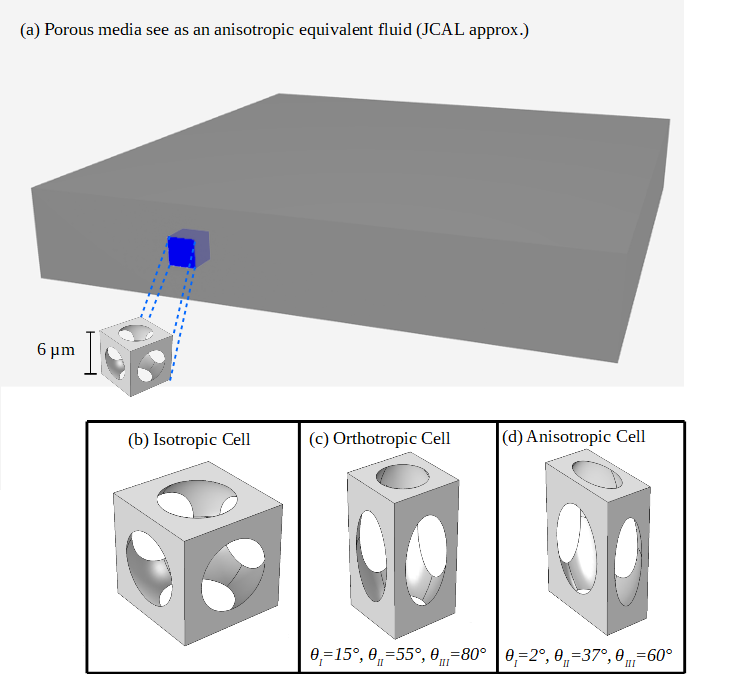
\includegraphics[scale=0.5]{Material_2.png}
        \caption{azerty}
        \label{Material}
    \end{figure}

The first parameter retrieve by the inverse method is the complex bulk modulus, as the three case of porous show the same bulk modulus and the method show very similar result for his identification, only the anisotropic case is represented on the figure (\ref{Grph_K}) as a global result for the three case.

    \begin{figure}[ht!]
        \centering
        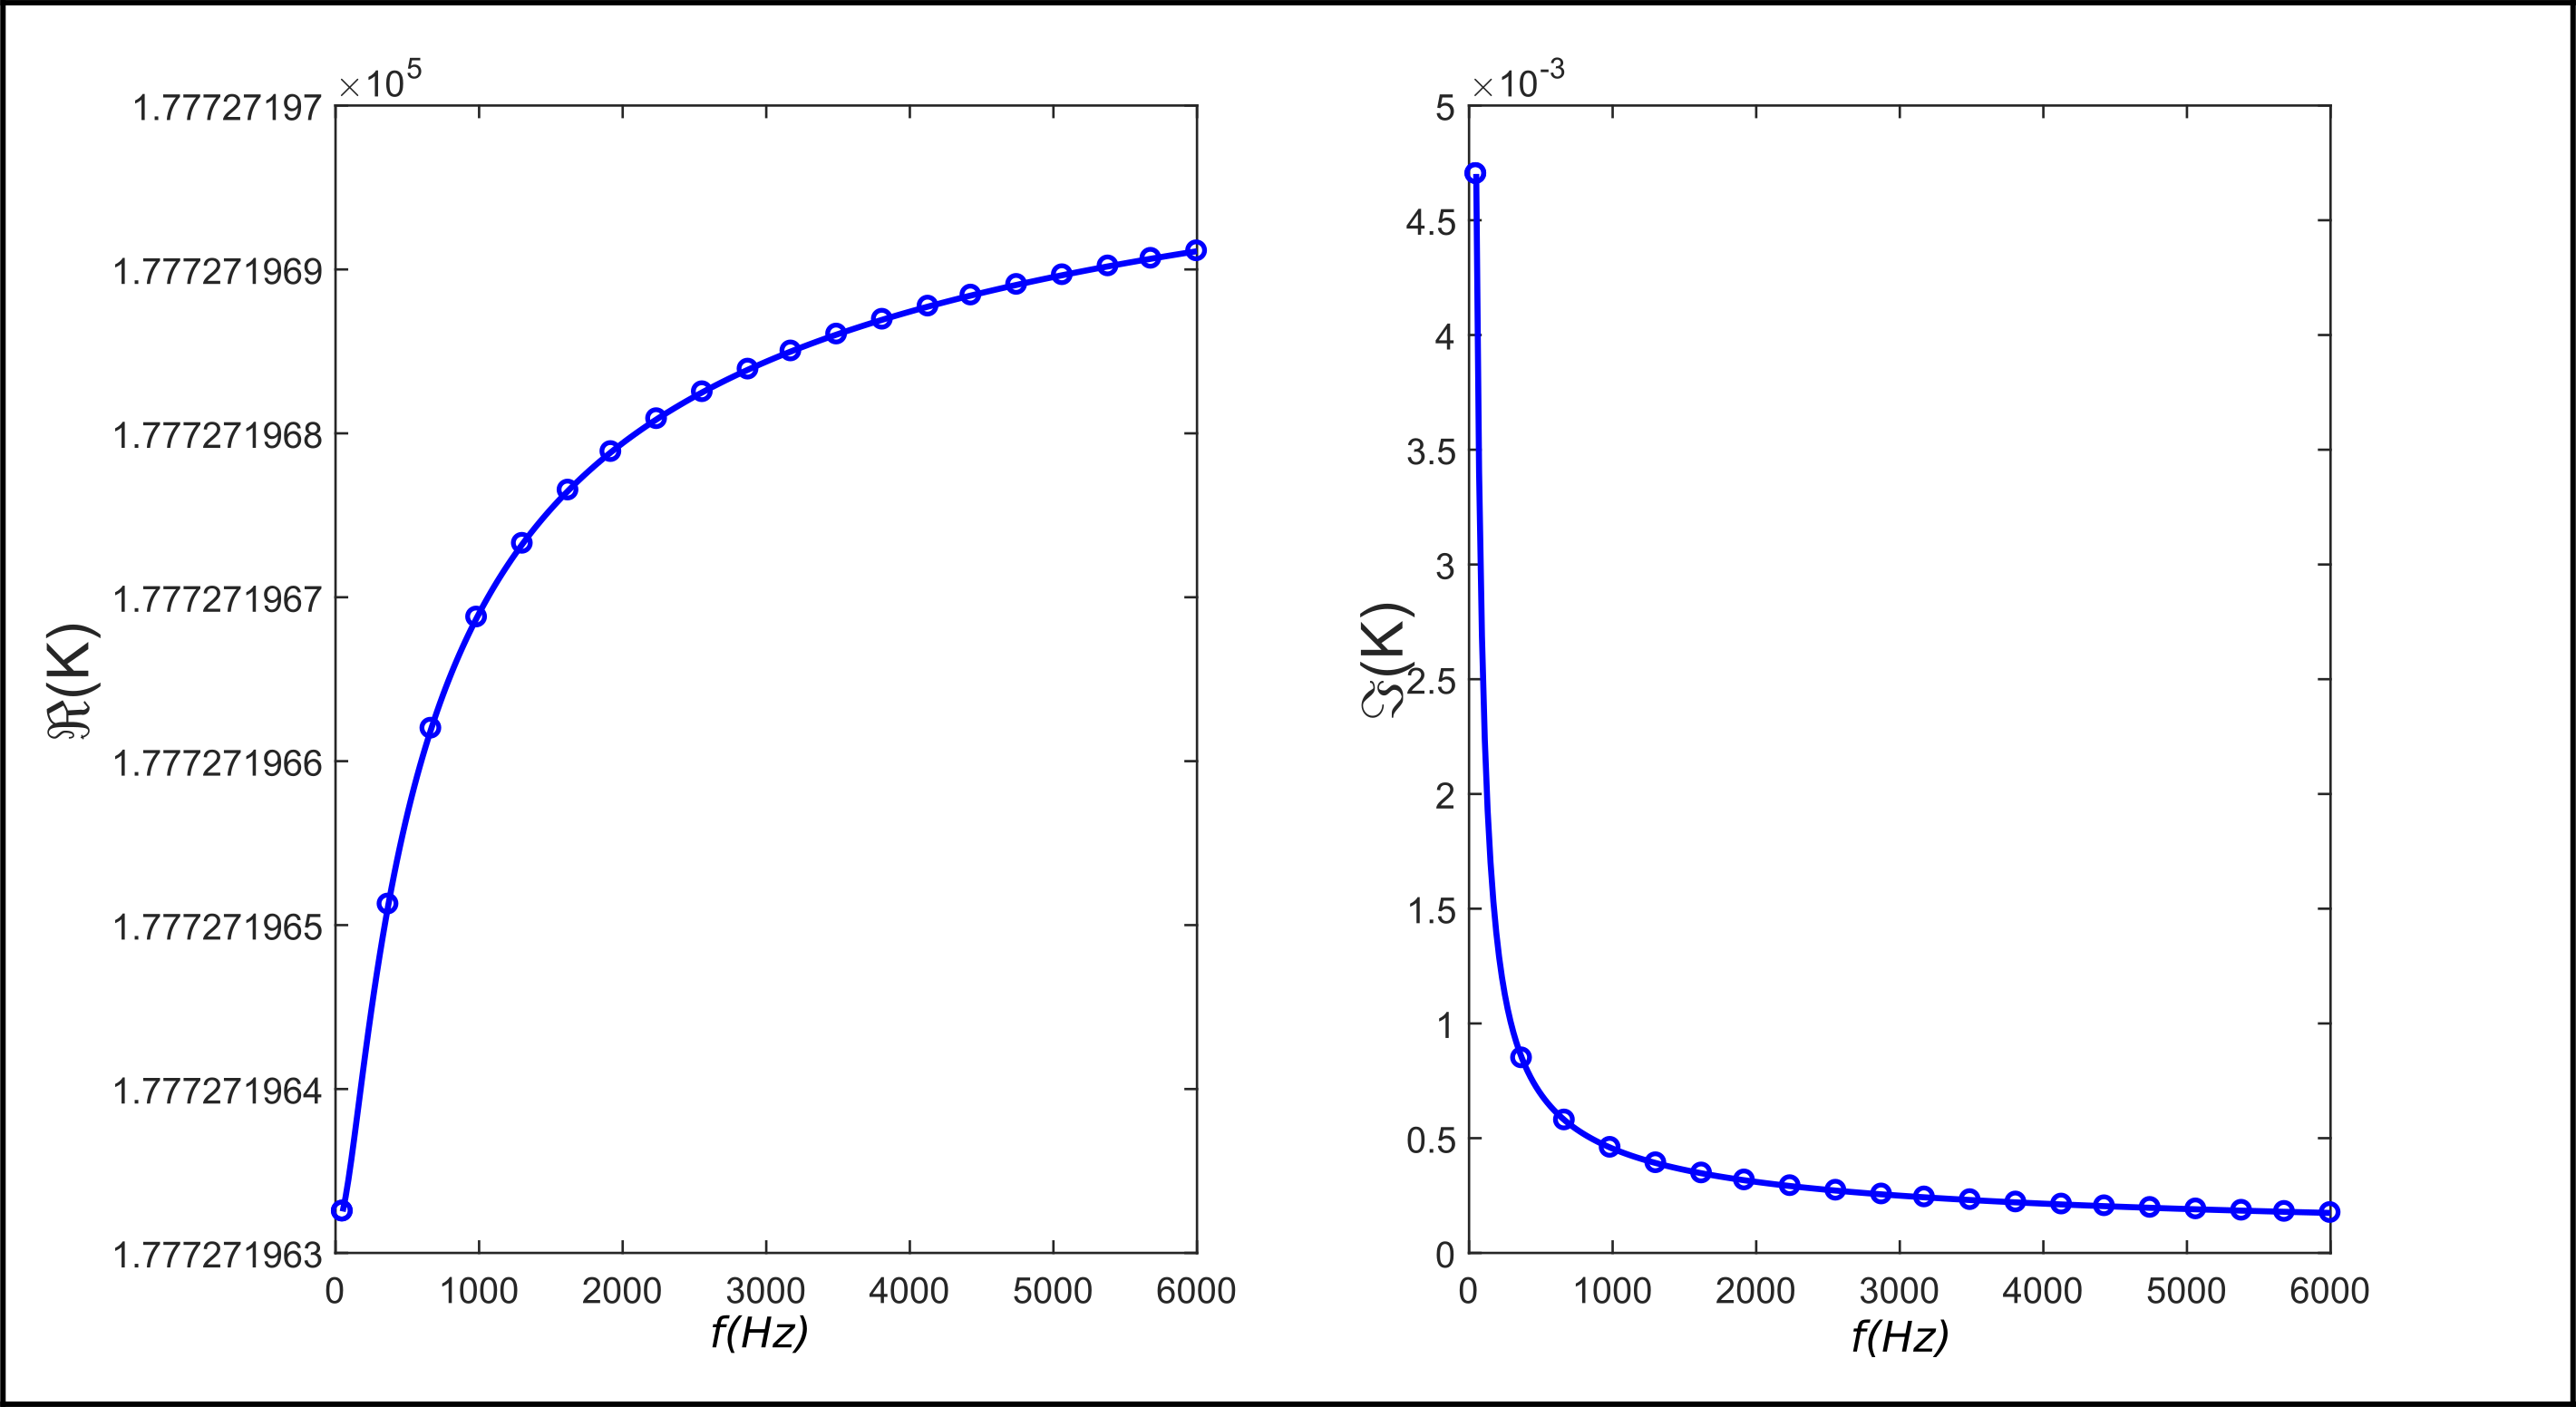
\includegraphics[scale=0.3]{Bulk.png}
        \caption{azerty}
        \label{Grph_K}
    \end{figure}
    
    As expect of a numerical validation, with no noise introduce in the model, the inverse method recover perfectly the bulk modulus value with a mean deviation of order $10^{-16}\%$ for the real part of K and $10^{-6}\%$ for the imaginary part. The 10-digit difference between the two part, is due to ... .
    
    Then the density are reconstruct base on the identified bulk modulus,  for the 3 case the obtained density are present on the figure (\ref{Grph_rho_rot}).
    \begin{figure}[ht!]
        \centering
        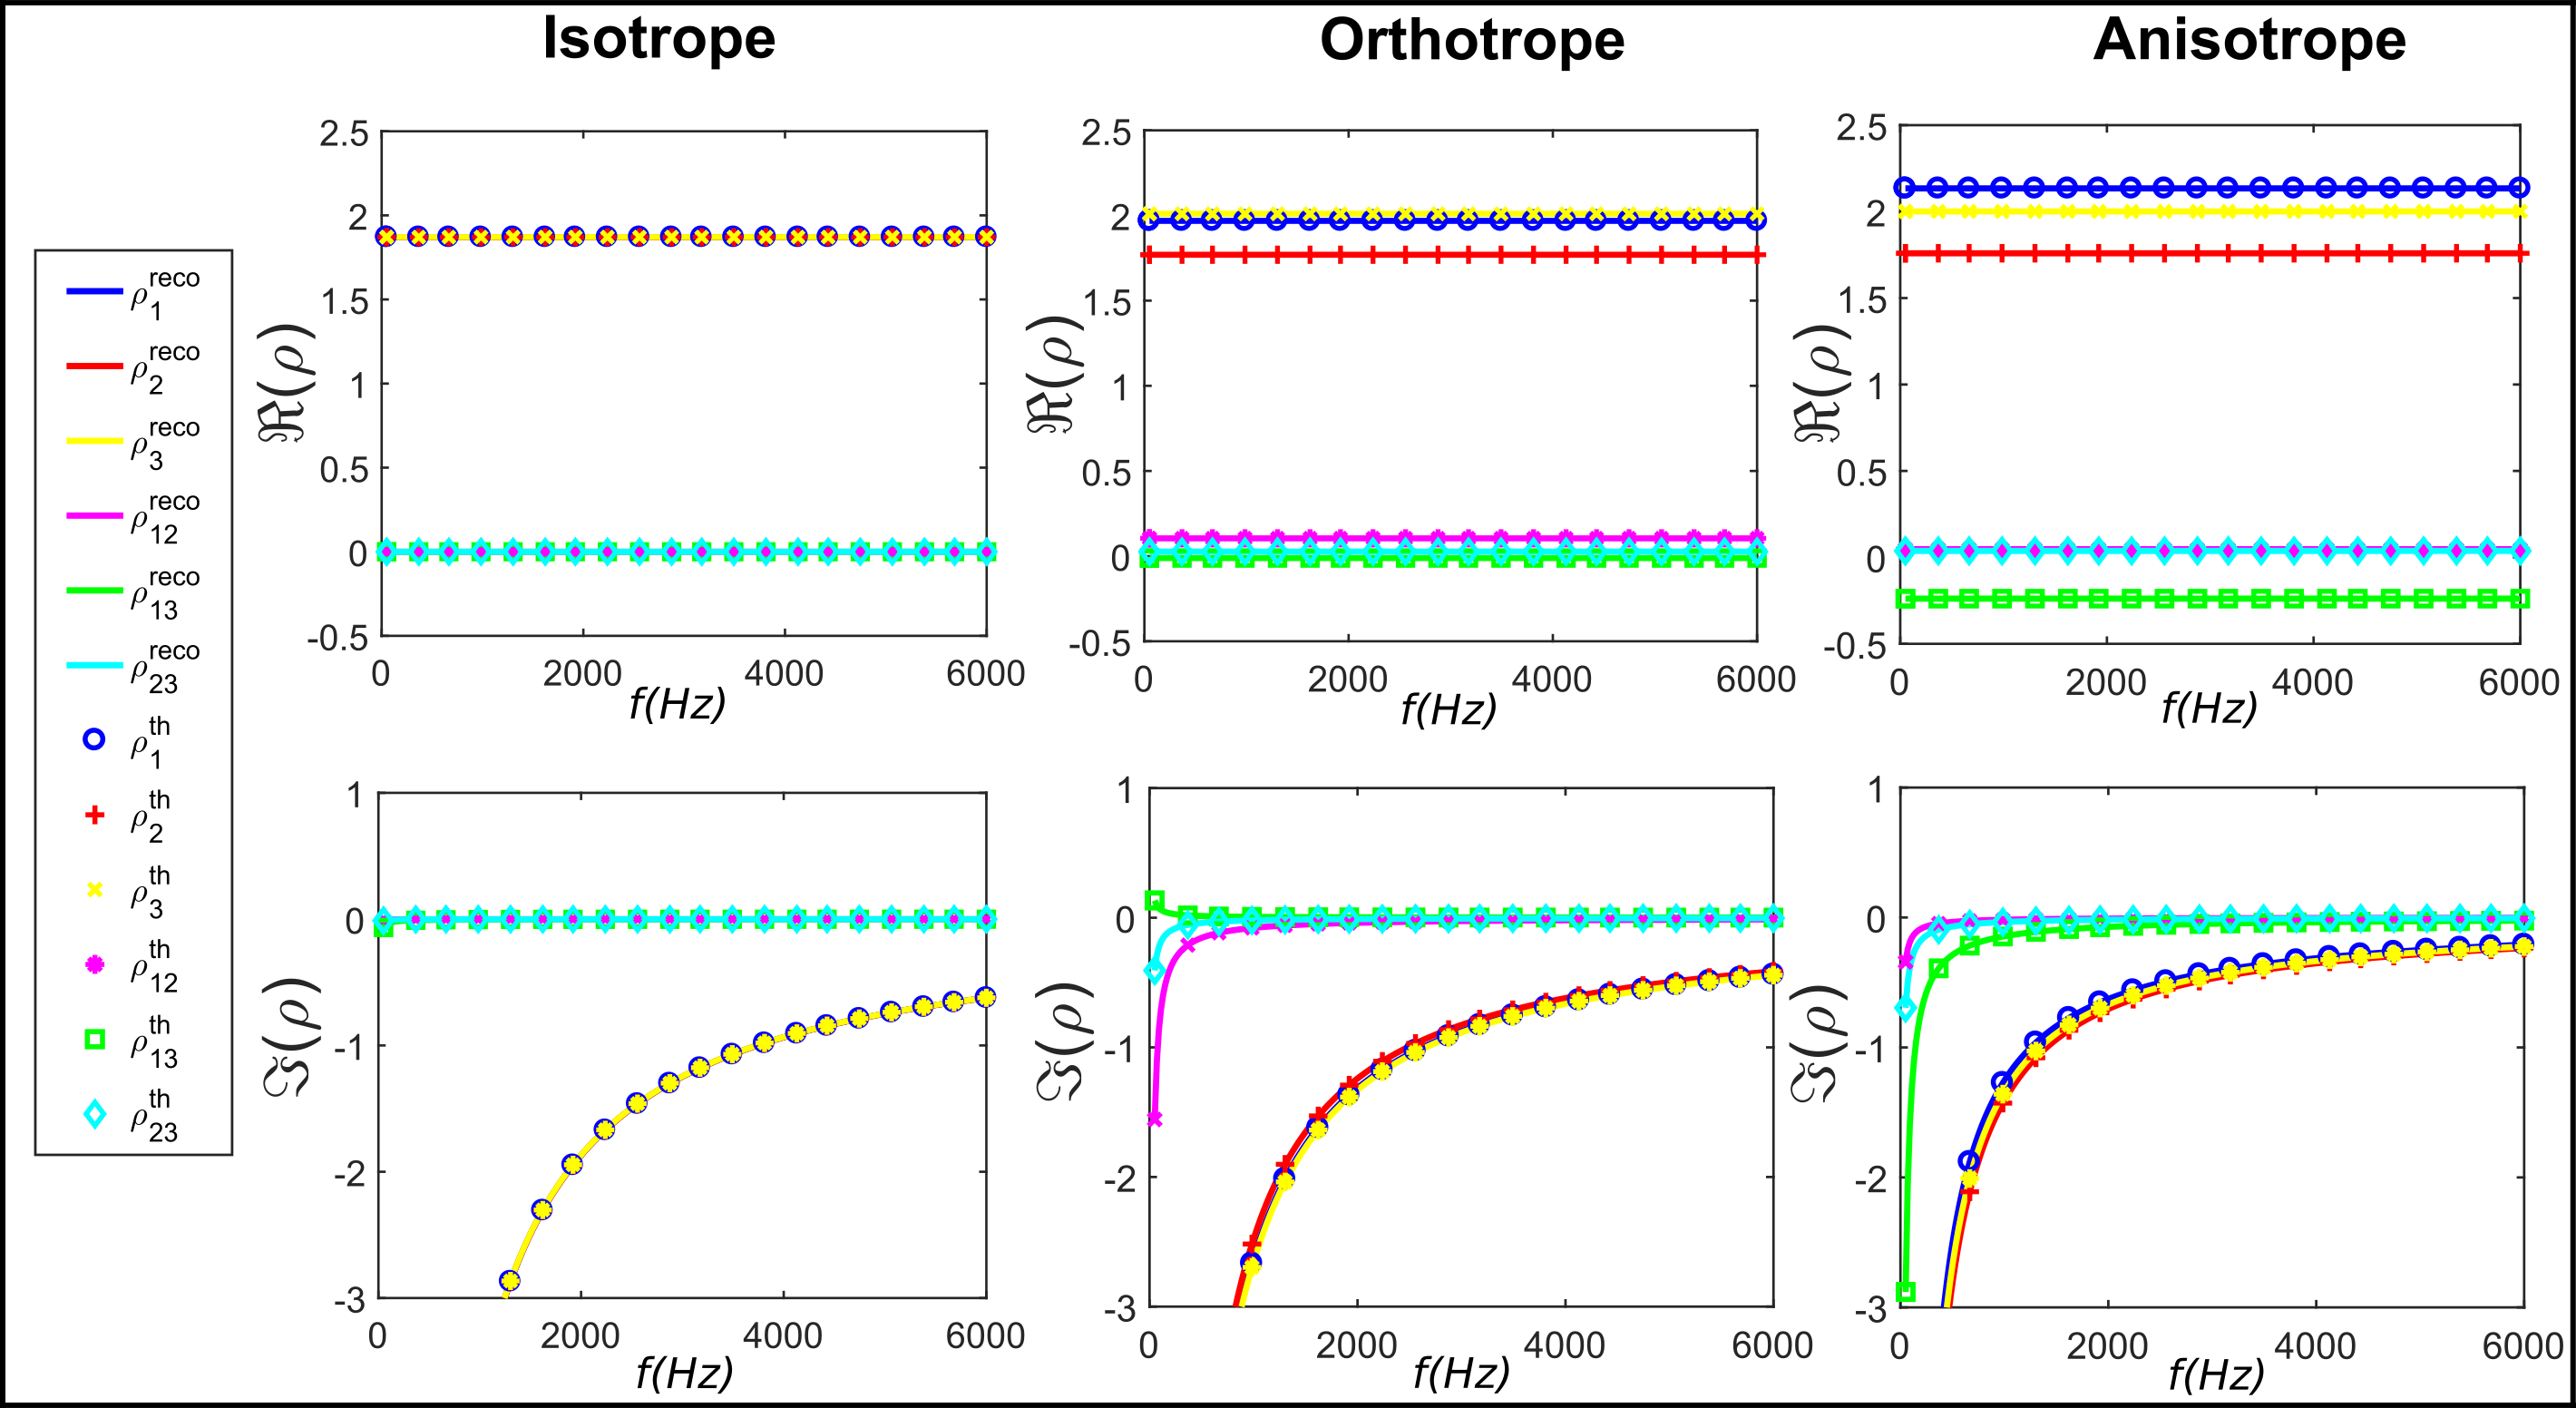
\includegraphics[scale=0.4]{Density_rot.png}
        \caption{azerty}
        \label{Grph_rho_rot}
    \end{figure}
    
    As the bulk modulus , the 6 complex density for the 3 case are well reconstruct and it's possible to recover the density of the porous material in his principal direction with a simple diagonalization of the density matrix (made by the eig function of matlab\copyright). One problem of this method is the arrangement of the eigen value, that need to be made, and can be different from the initial density in the principal direction. This unknown arrangement prevent from deriving the rotation of the principal direction.
    
    A convention is need to fix the arrangement of the eigen value, and to determine the rotation of the medium. The rotation is describe here by the three Euler angle, around successively $x_3$, $x_2$ and $x_1$, in configuration "ZYX". The fixed convention here is that both of  the rotation angle $\theta_I$ around $x_1$ and $\theta_{II}$ around $x_2$ should be contain between $0$ and $\frac{\pi}{2}$. After checking if the rotated base is direct, base who correspond to the eigen vector, successive permutation are operated until the condition on $\theta_I$ and $\theta_{II}$ are satisfied, then the permuted eigen vector is convert to euler angle (using the function rotm2eul of matlab\copyright).
    
    The figure (\ref{Grph_rho_dir}) present density and angle of rotation obtained.

    \begin{figure}[ht!]
        \centering
        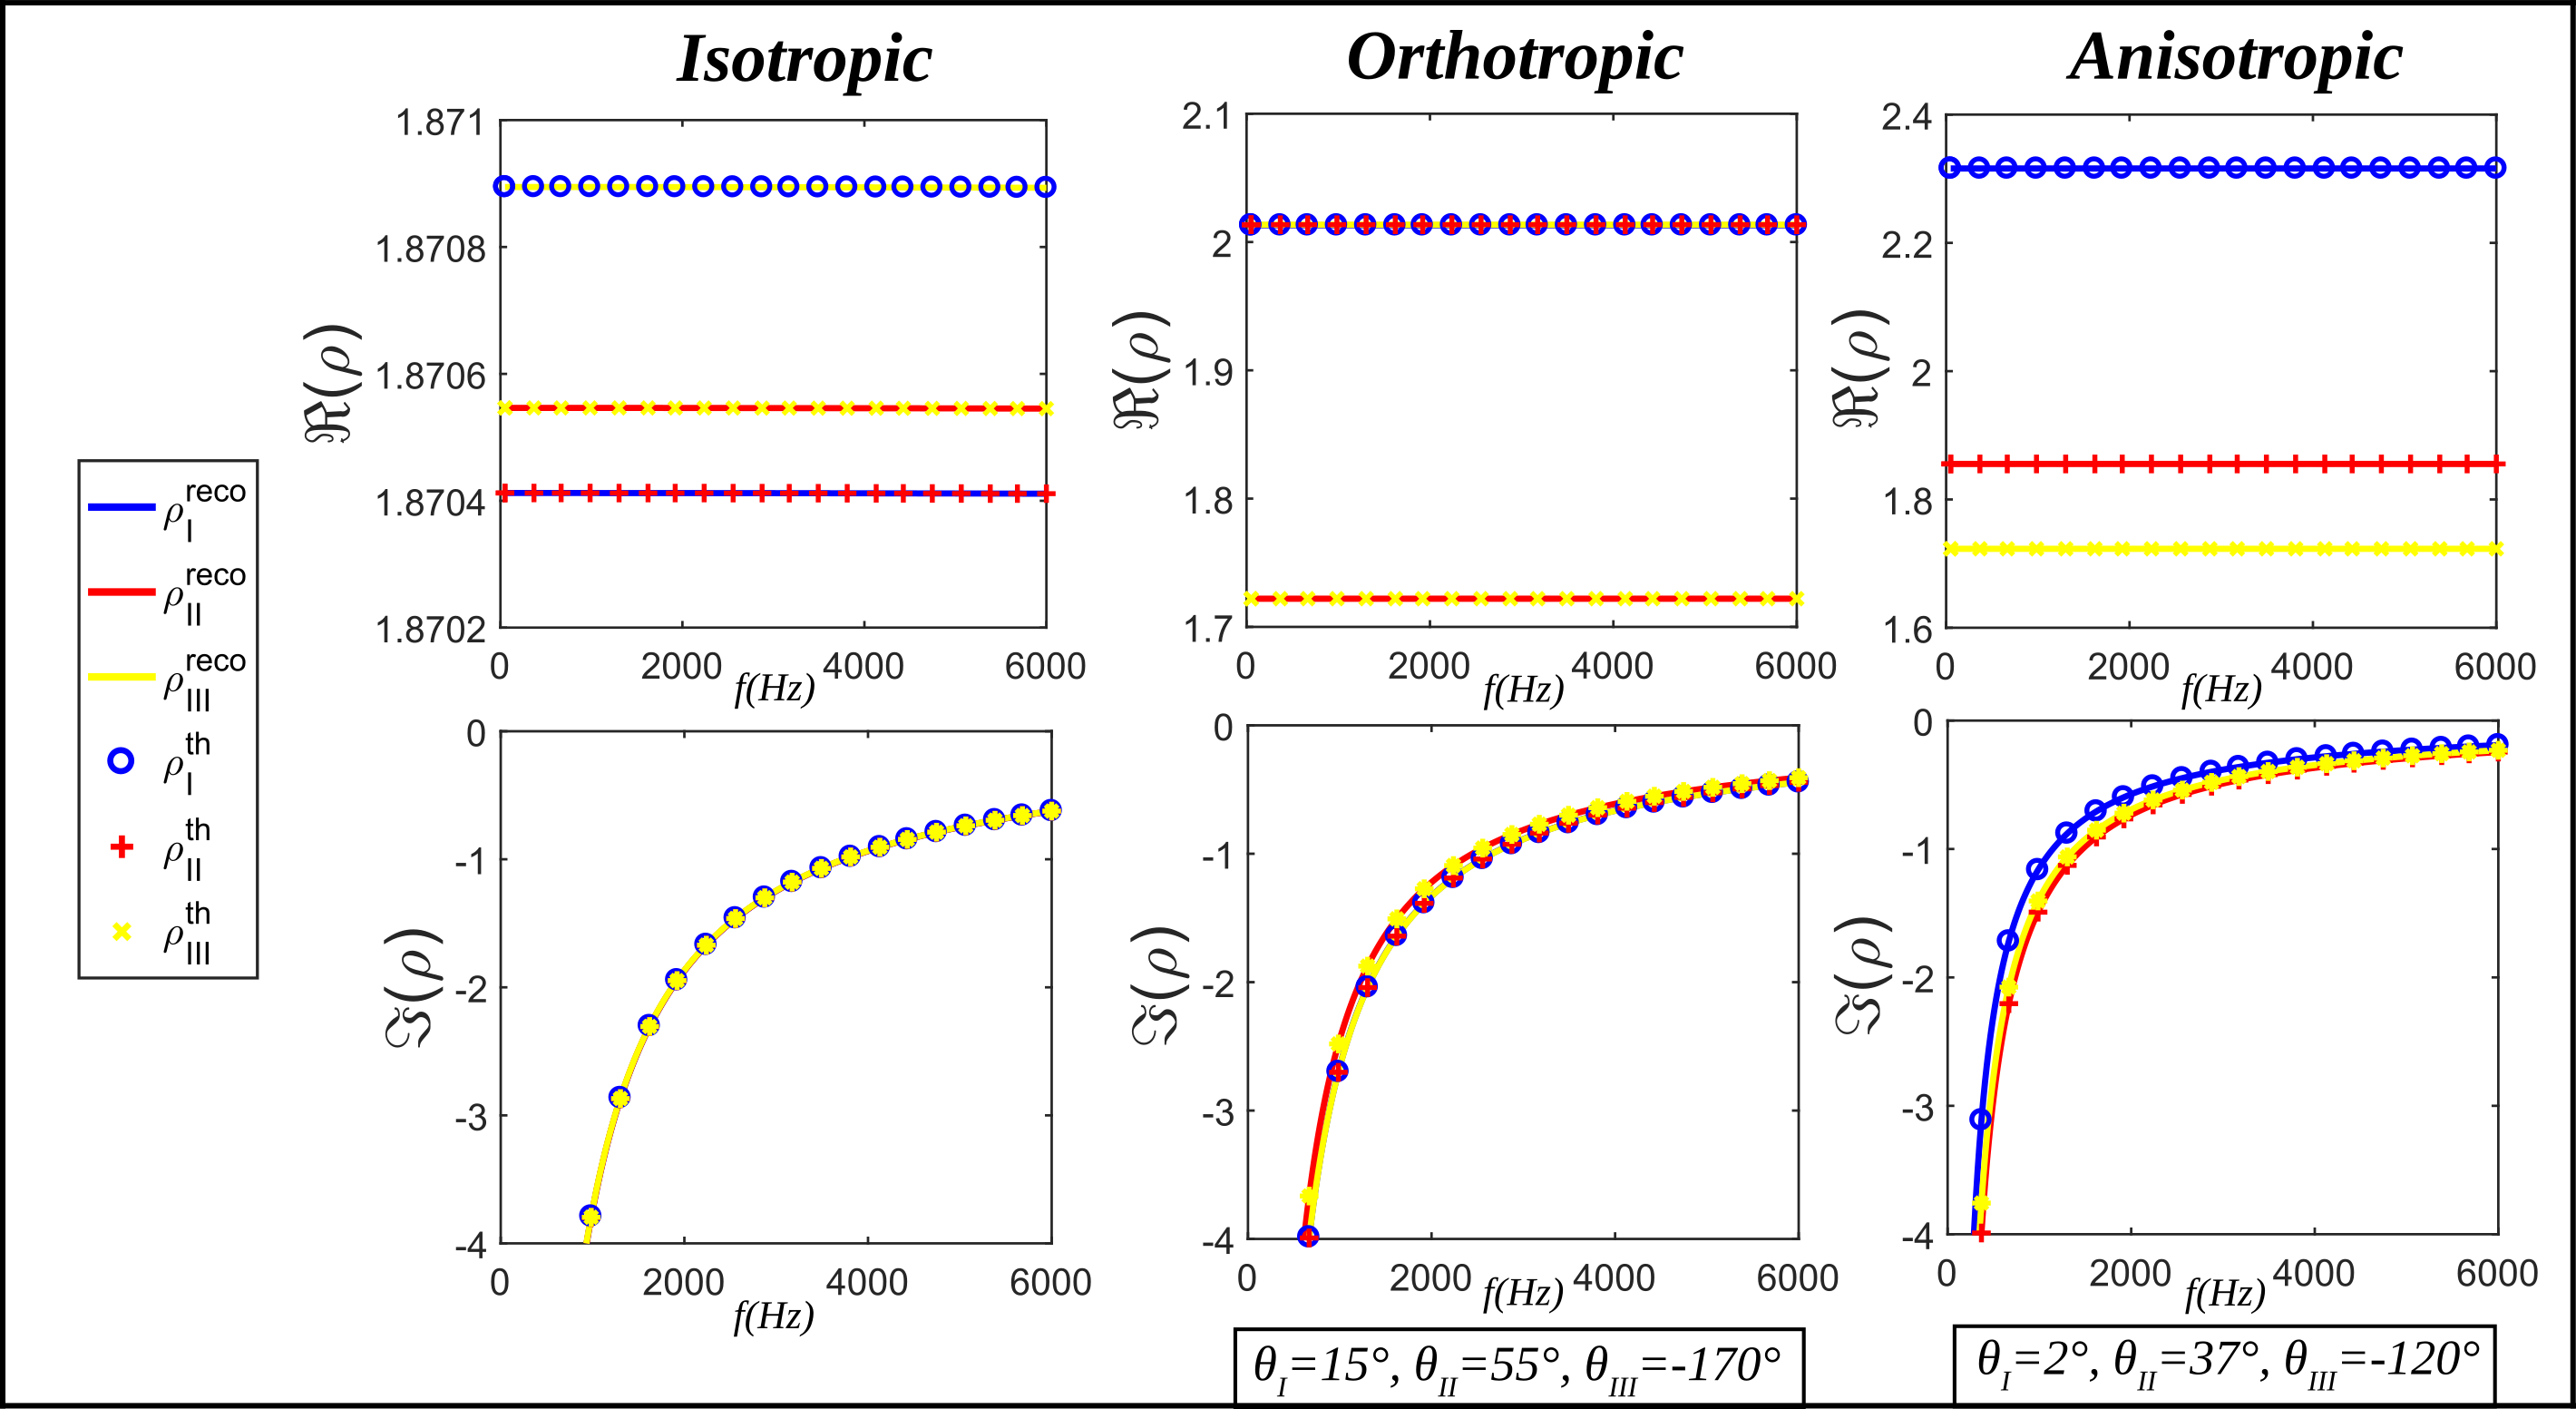
\includegraphics[scale=0.4]{Density_dir.png}
        \caption{azerty}
        \label{Grph_rho_dir}
    \end{figure}
    
    Three case are distinguish here, the first is the isotropic porous layer, it's easy too see that the reconstruct density matrix is the one of a isotropic material who correspond to the expect one, plus the homogeneization is done before rotating the layer, so here the roation is not observe whenever the egein value aren't arrange as the theroitical result expected.  For the second case, the orthotropic density are recover with an symmetry on the $x_1x_3$ plan instead of the theoritical symmetry on $x_1x_2$. This permutation of axis explain that the first two rotation angle $\theta_I$ and $\theta_{II}$ are recover perfectly but the third $\theta_{III}$ is shift of 90°, remind that a plan is $\pi$ periodic. The last case show anisotropic density, that identified the right density with the good arrangement. In this case the rotation angle are recover. 
    
%%%%%%%%%%%%%%%%%%%%%%%%%%%%%%%%%%%%%%%%%%%%%%%%%%%%%%%%%%%%%%%%%%%%%%
\section{Conclusion}


%%%%%%%%%%%%%%%%%%%%%%%%%%%%%%%%%%%%%%%%%%%%%%%%%%%%%%%%%%%%%%%%%%%%%%
\section{Annexe}
\subsection*{Propagation matrix $\bar{\bar{A}}$}
	From the expression (\ref{Euler1}), $v_1$ and $v_2$ can be express as a function of $p$ and $v_3$, so :
\begin{align*}
	v_1=\frac{1}{\rho_{11}-\frac{\rho_{12}^2}{\rho_{22}}}([\frac{k_1}{\omega}-\frac{\rho_{12}}{\rho_{22}}\frac{k_2}{\omega}]p+[\frac{\rho_{12}}{\rho_{22}}\rho_{23}-\rho_{13}]v_3), \\
	v_2=\frac{1}{\rho_{22}-\frac{\rho_{12}^2}{\rho_{11}}}([\frac{k_2}{\omega}-\frac{\rho_{12}}{\rho_{11}}\frac{k_1}{\omega}]p+[\frac{\rho_{12}}{\rho_{11}}\rho_{13}-\rho_{23}]v_3).
\end{align*}
 	Introducing this expression in (\ref{Euler2}) and (\ref{Euler3}), can be write $\frac{\partial}{\partial x_3}\bar{S}$ as $\frac{\partial}{\partial x_3}\bar{S}(p,v_3)$ :
    \begin{align*}
    \frac{\partial}{\partial x_3}v_3=&[\frac{i\omega}{K}-\frac{ik_1}{\rho_{11}-\frac{\rho_{12}^2}{\rho_{22}}}(\frac{k_1}{\omega}-\frac{\rho_{12}}{\rho_{22}}\frac{k_2}{\omega})-\frac{ik_2}{\rho_{22}-\frac{\rho_{12}^2}{\rho_{11}}}(\frac{k_2}{\omega}-\frac{\rho_{12}}{\rho_{11}}\frac{k_1}{\omega})]p\\
    &-[\frac{ik_1}{\rho_{11}-\frac{\rho_{12}^2}{\rho_{22}}}(\frac{\rho_{12}}{\rho_{22}}\rho_{23}-\rho_{13})+\frac{ik_2}{\rho_{22}-\frac{\rho_{12}^2}{\rho_{11}}}(\frac{\rho_{12}}{\rho_{11}}\rho_{13}-\rho_{23})]v_3,
    \end{align*}
    and 
    \begin{align*}
    \frac{\partial}{\partial x_3}p=&[\frac{i\omega \rho_{13}}{\rho_{11}-\frac{\rho_{12}^2}{\rho_{22}}}(\frac{k_1}{\omega}-\frac{\rho_{12}}{\rho_{22}}\frac{k_2}{\omega})+\frac{i\omega \rho_{23}}{\rho_{22}-\frac{\rho_{12}^2}{\rho_{11}}}(\frac{k_2}{\omega}-\frac{\rho_{12}}{\rho_{11}}\frac{k_1}{\omega})]p\\
    &+[\frac{i\omega \rho_{13}}{\rho_{11}-\frac{\rho_{12}^2}{\rho_{22}}}(\frac{\rho_{12}}{\rho_{22}}\rho_{23}-\rho_{13})+\frac{i\omega \rho_{23}}{\rho_{22}-\frac{\rho_{12}^2}{\rho_{11}}}(\frac{\rho_{12}}{\rho_{11}}\rho_{13}-\rho_{23})]v_3.
    \end{align*}
    Writing this two equation in matrix form, the expression (\ref{Matrice_complete}) can be obtain.
    
\subsection*{Reflection and transmission coefficients}
    To obtain the reflection and transmission coefficient, the transfer matrix $Tr$ and the boundary condition (\ref{BC_L}) and (\ref{BC_0}) are required.
    The expression of $Tr$ (\ref{Transfer_Matrix}) can be develop as :
     	\begin{align*}
 	Tr &=\bar{\bar{U}} \begin{pmatrix}
                         e^{-ik_{33}L} & 0 \\ 0 & e^{ik_{33}L}
                    \end{pmatrix} \bar{\bar{U^{-1}}}\\
     &= \frac{1}{2} \begin{pmatrix}
     					Z_3 & Z_3 \\ -1 & 1
      				\end{pmatrix} \begin{pmatrix}
                                   	e^{-ik_{33}L} & 0 \\ 0 & e^{ik_{33}L}
                                   \end{pmatrix} \begin{pmatrix}
     												\frac{1}{Z_3} & -1 \\ \frac{1}{Z_3} & 1
      											 \end{pmatrix}\\
    &=\frac{1}{2} \begin{bmatrix}
    				e^{ik_{33}L}+e^{-ik_{33}L} & Z_3(e^{ik_{33}L}-e^{-ik_{33}L}) \\ 
    				\frac{e^{ik_{33}L}-e^{-ik_{33}L}}{Z_3} & e^{ik_{33}L}+e^{-ik_{33}L}
    				\end{bmatrix}\\
 	&= \begin{bmatrix}
    				cos(k_{33}L) & i Z_3 sin(k_{33}L) \\ 
    				i\frac{sin(k_{33}L)}{Z_3} & cos(k_{33}L)
    	\end{bmatrix}.
    \end{align*}
    Introducing the new transfer matrix in the equation (\ref{PB}), the two next equation come :
    
    \begin{align}
    (1+R)&=[cos(k_{33}L)-i\frac{Z_3}{Z} sin(k_{33}L)]T,\label{T_cal1} \\ 
    -\frac{(1-R)}{Z}&=[-\frac{cos(k_{33}L)}{Z}+i\frac{sin(k_{33}L)}{Z_3}].\label{T_cal2}
    \end{align}
    
    And resolving the system of 2 equation with 2 unknown, the reflection and transmission coefficient (\ref{Transmission}) and (\ref{Reflexion}) can be obtain.
    
\subsection*{$\rho_1$, $\rho_2$ and $\rho_{12}$ determination}
    To determine the three densities $\rho_1$, $\rho_2$ and $\rho_{12}$, it's proposed to resolve the system of 3 equation with 3 unknown  [(\ref{Comp_1}):(\ref{Comp_3})], three ratio of densities can be defined as : 
    
    \begin{align}
    &\frac{(\ref{Comp_2})}{(\ref{Comp_1})} :\ \frac{\rho_1}{\rho_2}=\frac{\gamma'|^{(\frac{\pi}{6})}_{(0)}}{\gamma'|^{(\frac{\pi}{6})}_{(\frac{\pi}{2})}}=X_1,\label{Comp_rho2_rho1} \\
    &\frac{(\ref{Comp_1})+(\ref{Comp_2})-(\ref{Comp_3})}{(\ref{Comp_2})} :\ \frac{\rho_{12}}{\rho_1}=\frac{1}{2}\frac{\gamma'|^{(\frac{\pi}{6})}_{(0)}+\gamma'|^{(\frac{\pi}{6})}_{(\frac{\pi}{2})}-\gamma'|^{(\frac{\pi}{4})}_{(\frac{\pi}{4})}}{\gamma'|^{(\frac{\pi}{6})}_{(\frac{\pi}{2})}}=X_2,\label{Comp_rho12_rho1} \\
    &\frac{(\ref{Comp_1})+(\ref{Comp_2})-(\ref{Comp_3})}{(\ref{Comp_1})} :\ \frac{\rho_{12}}{\rho_2}=\frac{1}{2}\frac{\gamma'|^{(\frac{\pi}{6})}_{(0)}+\gamma'|^{(\frac{\pi}{6})}_{(\frac{\pi}{2})}-\gamma'|^{(\frac{\pi}{4})}_{(\frac{\pi}{4})}}{\gamma'|^{(\frac{\pi}{6})}_{(0)}}=X_3.\label{Comp_rho12_rho2}
    \end{align}
    
    And by introducing the expression [(\ref{Comp_rho2_rho1}):(\ref{Comp_rho12_rho2})] in (\ref{Comp_1}, the equation can be express in function of $\rho_2$, so :
    \begin{align}
    \rho_2=\frac{X_1}{(X_1-X_3^2)\gamma'|^{(\frac{\pi}{6})}_{(\frac{\pi}{2})}}.\label{comp_rho2}
    \end{align}
    Developed, it come the expression (\ref{rho2})
    Considering $\rho_1=X_1\rho_2$ and $\rho_{12}=X_3\rho_2$, the expression (\ref{rho1}) and (\ref{rho12}) can be obtain.
    

\end{document}
